\begin{figure}
\centering
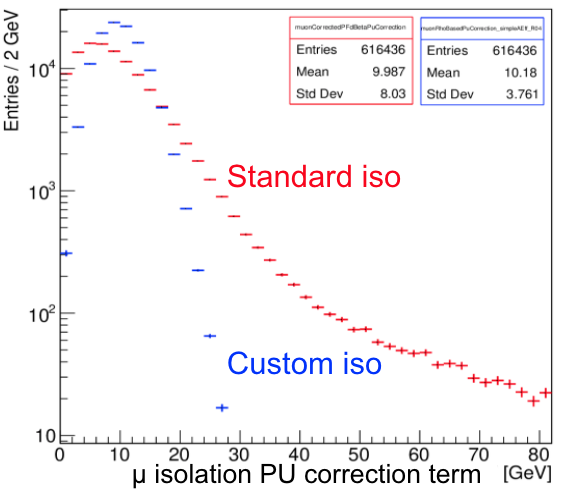
\includegraphics[width=0.44\textwidth]{figures/selection/CustomVsStandardMuIsoPUcorrection_2018emuTTbar_PCR.png}
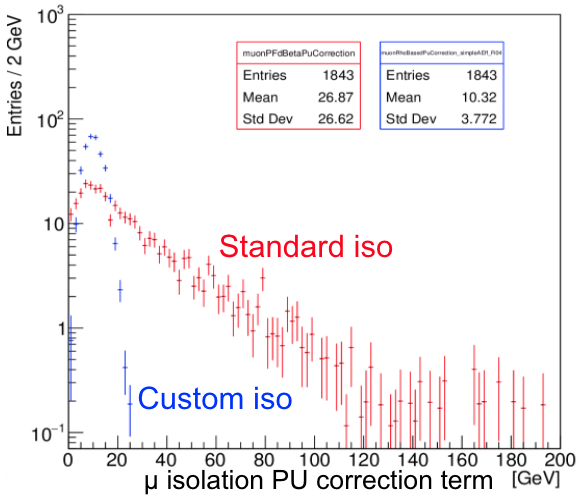
\includegraphics[width=0.45\textwidth]{figures/selection/CustomVsStandardMuIsoPUcorrection_2018emuTTbar_500To1000um.png}
\caption{The muon isolation pileup correction term, for the standard muon isolation and the modified muon isolation in simulated \ttbar events that pass the $\Pe\Pgm$ preselection in 2018 conditions. The plot on the left is for muon $\ad<\SI{100}{\um}$, and the plot on the right is for muon $500<\ad<\SI{1000}{\um}$.}
\label{iso_pu_term_comparison}
\end{figure}

\begin{figure}\fxnote{weirdly low resolution}
\centering
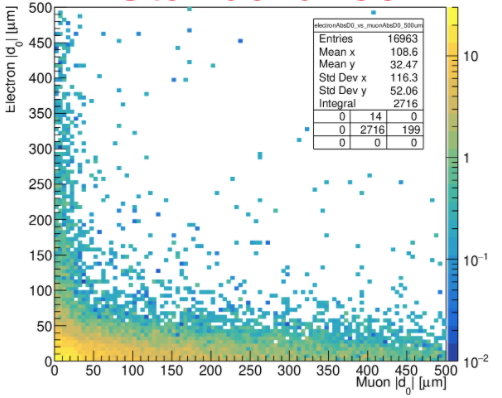
\includegraphics[width=0.45\textwidth]{figures/selection/StandardIso_ElectronD0vsMuonD0_2018emuTTbar.png}
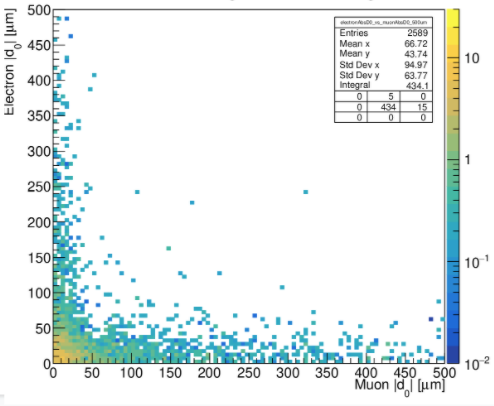
\includegraphics[width=0.44\textwidth]{figures/selection/CustomIso_ElectronD0vsMuonD0_2018emuTTbar.png}
\caption{The electron \ad versus the muon \ad, for \ttbar simulated events that pass the $\Pe\Pgm$ preselection and where at least one lepton comes from a heavy-flavor meson. The plot on the left uses the standard isolation, and the plot on the right uses the modified isolation.}
\label{iso_performance_comparison}
\end{figure}

\begin{figure}\fxnote{weirdly low resolution}
\centering
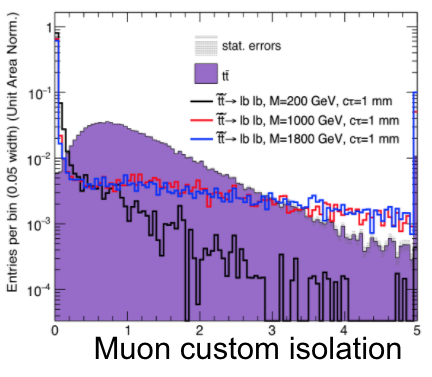
\includegraphics[width=0.5\textwidth]{figures/selection/MuonCustomIso_TTbar_Signal.png}
\caption{The muon custom isolation distribution for simulated \ttbar background and \stoptolb signal events in 2018 conditions\fxnote{specify selection}.}
\label{iso_signal_bg}
\end{figure}